\chapter{Simulations}
\label{chapter:simulations}
\section{Introduction to Simulations}
Simulating the various sub-circuits of the amplifier system is crucial to minimize unnecessary trial and error. Utilizing circuit simulation software, such as LTSpice, offers valuable insights into the system's behaviour that go beyond what can be achieved through manual calculations. Simulations enable the creation of different plots, which help validate and reinforce design decisions.

\section{Simulations and Results}


\subsection{Power Supply}
\subsubsection{Simulated Power Supply Analysis}
Analysis of the LTSpice simulations was initialized using the values partially gained from calculations \ref{DischargeResistor} and \ref{CapacitanceEquation}, although real-world availability of these values wasn't possible. Therefore, deviations were made from the values presented previously; for the capacitor, a value of 6800$\mu$F was chosen (limited by the range of available smoothing capacitor values and considerations related to inrush current) since a higher capacitance results in a lower ripple percentage. A value of 3.9k$\Omega$ was chosen for the discharge resistors since a smaller resistance results in a shorter discharge time after the operation and minimizes the risk of excessive power dissipation that could potentially damage the resistor when using even smaller values, and due to other previously mentioned effects with the sizing of discharge resistors, where the discharge resistance could have influenced the ripple voltage, even if this effect would be negligible.
\begin{figure}[H]
    \centering
    \captionsetup{justification=raggedright, labelfont=bf}
    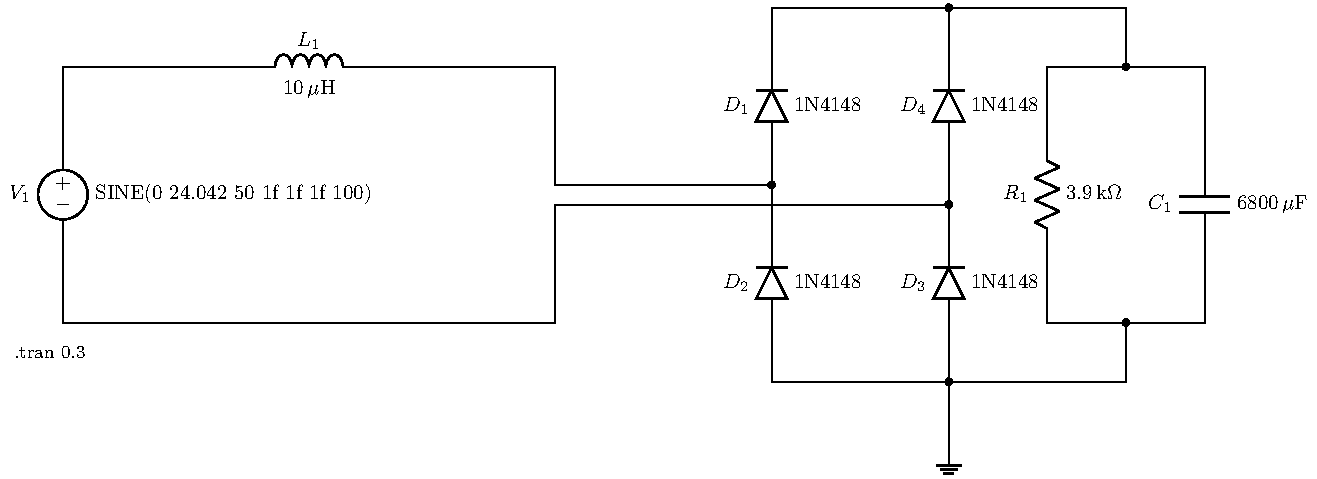
\includegraphics[width=0.8\linewidth]{TU Delft Booming Bass Project Report/figures/PowerSupply/MainPowerSupplyLTSPice.pdf}
    \caption{{LTSpice circuit. For simplicity, only one side of the power supply design is considered, as the transformer is symmetrical on its output terminals. A voltage source is employed at $V_1$ to represent the input voltage (230V,50Hz) with (24.42V, 50Hz) as the specified parameters. This configuration ensures that the resultant voltage and current after the rectification process are consistent with the behavior of a properly modelled transformer.}}
    \label{fig:MainPowerSupplySchematicLTSpice}
\end{figure}

As previously discussed, the LTSpice simulations were performed for only one output terminal, as the use of a center-tapped transformed allows the existence of symmetry of the power supply; this ensures consistent behaviour on both the positive and negative output terminals. This means that analysis on only one side of the output terminal is sufficient. Next to that, the transformer was replaced by an AC voltage source with an inductor in series to model the non-ideal transformer. The model of the circuit used in LTSpice can be seen in \sfautoref{fig:MainPowerSupplySchematicLTSpice}.

\begin{figure}[H]
    \centering
    \captionsetup{justification=raggedright, labelfont=bf}
    \resizebox{0.9\columnwidth}{!}{%
        \begin{tikzpicture} 
            \pgfplotsset{
                every axis legend/.append style={at={(0.98,0.02)}, anchor=south east, legend columns=1},
                every axis/.append style={
                    grid=major,
                    grid style={line width=0.5pt, draw opacity=0.4},
                    tick align=inside, % Ticks will now be inside the plot
                    minor tick num=5
                }
            }
            \begin{axis} [
                xlabel={Time [s]}, % Adjusted x-axis label
                ylabel={$V_{\text{out}}$ [V]},
                title={Effect of different load resistances on $V_{\text{out}}$},
                width=\textwidth,
                height=0.6\textwidth,
                xticklabel style={/pgf/number format/.cd, fixed, precision=3}, % Force fixed-point notation
                scaled x ticks=false, % Disable automatic scaling
                xtick scale label code/.code={}, % Ensure no scale label is shown
                enlargelimits=true % Ensure the graph has enough space for ticks
            ]
                % Plot with 19Ω
                \addplot+[black, no markers] 
                    table [x=time, y=V(n001), col sep=comma] 
                    {TU Delft Booming Bass Project Report/appendix/csv/sim/filtered19ohm_data.txt};
                \addlegendentry{$V_{\text{out}}$ with 19$\Omega$}

                % Plot with 38Ω
                \addplot+[blue, no markers] 
                    table [x=time, y=V(n001), col sep=comma] 
                    {TU Delft Booming Bass Project Report/appendix/csv/sim/filtered38ohm_data.txt};
                \addlegendentry{$V_{\text{out}}$ with 38$\Omega$}

                % Plot with 76Ω
                \addplot+[red, no markers] 
                    table [x=time, y=V(n001), col sep=comma] 
                    {TU Delft Booming Bass Project Report/appendix/csv/sim/filtered76ohm_data.txt};
                \addlegendentry{$V_{\text{out}}$ with 76$\Omega$}

                % Plot with no load
                \addplot+[green, no markers] 
                    table [x=time, y=V(n001), col sep=comma] 
                    {TU Delft Booming Bass Project Report/appendix/csv/sim/filterednoload2_data.txt};
                \addlegendentry{$V_{\text{out}}$ with no load}
            \end{axis}
        \end{tikzpicture}%
    }

    \caption{The simulated circuit output voltage for different load resistances. The black line represents the circuit with 19$\Omega$, the blue line with 38$\Omega$, the red line with 76$\Omega$, and the green line with no load.}
    \label{fig:OutputVoltageWith-Without}
\end{figure}


\begin{figure}[H]
    \centering
    \begin{minipage}{0.48\textwidth}
        \centering
        \captionsetup{justification=raggedright, labelfont=bf}
        \caption{Simulation characteristics of the power supply under varying load levels, displaying the average output voltage, current, and ripple percentage for each load condition. A graphical representation of this data is shown in \sfautoref{fig:OutputVoltageRipplePower}. The results highlight the performance of the power supply across different load resistances, with notable variations in ripple percentage and system stability as the load conditions change.}
        \begin{threeparttable}
          \centering
          \begin{tabular}{c @{\hspace{12pt}} *4{c} S @{\hspace{12pt}}}
            \toprule
            \multicolumn{5}{c}{\textbf{Simulated Power Supply Characteristics}} \\
            \cmidrule(lr){1-5}
            & & \multicolumn{3}{c}{\textbf{Performance Metrics}} \\
            \cmidrule(lr){3-5}
            & $R_\text{Load}$ [$\Omega$] & $V_\text{Av.}$ [V] & $I_\text{res}$ [A] & $u_\text{ripple}$ [\%] \\
            \midrule
            1 & 19 & 18.3 & 0.963 & 2.58 \\
            2 & 38 & 19.6 & 0.516 & 1.43 \\
            3 & 76 & 20.5 & 0.27 & 0.78 \\
            4 & Open & 22.3 & 0.00 & 0.55 \\
            \bottomrule
          \end{tabular}
        \end{threeparttable}
        
        \label{tab:CharacteristicsSim}
    \end{minipage}\hfill
    \begin{minipage}{0.48\textwidth}
        \centering
        \resizebox{\linewidth}{!}{%
            \begin{tikzpicture} 
                \pgfplotsset{
                    every axis legend/.append style={ at={(0.02,0.98)}, anchor=north west, legend columns = 1}, 
                    every axis/.append style={ytick distance=0.5, xtick distance=2, minor tick num=1, grid=major,
                    every axis grid/.append style={line width=0.5pt, draw opacity=0.4}}}
                    \begin{axis} [xlabel = {Delivered power [W]}, ylabel = {Ripple [\%]}]
                        \addlegendentry{Ripple [\%]}
                        \addplot+[no markers] table[row sep=crcr] {
                            {Supplied Power (W):}       {Ripple(\%):} \\
                            17.63       2.58  \\
                            10.11     1.43  \\
                            5.54     0.78  \\
                            0     0.55  \\
                        };
                    \end{axis}
            \end{tikzpicture}%
        }
        \captionsetup{justification=raggedright, labelfont=bf}
        \caption{The output voltage ripple as a function of the power delivered to varying load resistances, illustrating and highlighting the variations in ripple in response to changes in load power.}
        \label{fig:OutputVoltageRipplePower}
    \end{minipage}
\end{figure}

Table \ref{tab:CharacteristicsSim} presents the simulation results for the power supply operating under different resistive load conditions. The presented data includes each load scenario's corresponding average output voltage, current, and ripple percentage. The ripple percentage was determined using \seautoref{RippleVoltageEquation}. All the values were obtained through computational analysis, with the detailed code provided in the appendix. These results offer a comprehensive evaluation of the power supply's performance across different load levels, highlighting its capability to deliver stable output and maintain consistent performance under varying operating conditions.
\begin{figure}[H]
    \centering
    \captionsetup{justification=raggedright, labelfont=bf}
    \resizebox{0.9\columnwidth}{!}{%
        \begin{tikzpicture} 
            \pgfplotsset{
                every axis legend/.append style={at={(0.98,0.02)}, anchor=south east, legend columns=1},
                every axis/.append style={
                    grid=major,
                    grid style={line width=0.5pt, draw opacity=0.4},
                    tick align=inside, % Ticks will now be inside the plot
                    minor tick num=5
                }
            }
            \begin{axis} [
                xlabel={Time [s]}, % Adjusted x-axis label
                ylabel={$V_{\text{out}}$ [V]},
                title={Effect of the smoothing capacitors on $V_{\text{out}}$},
                width=\textwidth,
                height=0.6\textwidth,
                xticklabel style={/pgf/number format/.cd, fixed, fixed zerofill, precision=3}, % Force fixed-point notation
                scaled x ticks=false, % Disable automatic scaling
                xtick scale label code/.code={}, % Ensure no scale label is shown
                enlargelimits=true % Ensure the graph has enough space for ticks
            ]
                % Plot with capacitors
                \addplot+[black, no markers] 
                    table [x={time}, y={V(n001)}, col sep=comma, mark=none] 
                    {TU Delft Booming Bass Project Report/appendix/csv/sim/filtered_data.txt};
                \addlegendentry{$V_{\text{out}}$ with capacitors}
                
                % Plot without capacitors
                \addplot+[blue, no markers] 
                    table [x={time}, y={V(n005)}, col sep=comma, mark=none] 
                    {TU Delft Booming Bass Project Report/appendix/csv/sim/filtered_data.txt};
                \addlegendentry{$V_{\text{out}}$ without capacitors}
            \end{axis}
        \end{tikzpicture}%
    }

    \caption{{The simulated circuit output voltage. The blue line represents the circuit without smoothing capacitors, while the black line shows the circuit with the 6.8$\mu$F smoothing capacitors in place.}}
    \label{fig:OutputVoltageWith-Without}
\end{figure}

Without a smoothing capacitor, the full-wave rectified waveform exhibits a ripple, with oscillations in voltage that follow the rectified signal. The absence of smoothing capacitors results in "negative" voltage dips between the peaks, as the diode stops conducting the during rectification process, creating a brief dip to zero or even negative. These negative voltages, as seen in Fig. \ref{fig:OutputVoltageWith-Without}, could also arise from minor errors or deviations in the measurement setup. Additionally, the behavior of the diodes may contribute to these negative readings. When the input voltage is near zero, the forward voltage drop of the diodes can cause the output to become negative until the input voltage exceeds the threshold required for conduction. This results in small negative spikes, particularly under low load or near-zero input conditions.
\begin{figure}[H]
    \centering
    \captionsetup{justification=raggedright, labelfont=bf}
    \resizebox{0.9\columnwidth}{!}{%
        \begin{tikzpicture} 
            \pgfplotsset{
                every axis legend/.append style={at={(0.98,0.02)}, anchor=south east, legend columns=1},
                every axis/.append style={
                    grid=major,
                    grid style={line width=0.5pt, draw opacity=0.4},
                    tick align=inside, % Ticks will now be inside the plot
                    minor tick num=5
                    }
            }
            \begin{axis} [
                title={Effect of the smoothing capacitors on $I_T$},
                xlabel={Time [s]},
                ylabel={$I_T$ [A]},
                width=\textwidth,
                height=0.6\textwidth,
                xticklabel style={/pgf/number format/.cd, fixed, fixed zerofill, precision=3}, % Force fixed-point notation
                scaled x ticks=false, % Disable automatic scaling
                xtick scale label code/.code={}, % Ensure no scale label is shown
                enlargelimits=true % Ensure the graph has enough space for ticks
            ]
                % Plot with capacitors
                \addplot+[black, no markers] 
                    table [x={time}, y={I(L1)}, col sep=comma, mark=none] 
                    {TU Delft Booming Bass Project Report/appendix/csv/sim/filteredcurrent_data.txt};
                \addlegendentry{$I_T$ with capacitors}
                
                % Plot without capacitors
                \addplot+[blue, no markers] 
                    table [x={time}, y={I(L2)}, col sep=comma, mark=none] 
                    {TU Delft Booming Bass Project Report/appendix/csv/sim/filteredcurrent_data.txt};
                \addlegendentry{$I_T$ without capacitors}
            \end{axis}
        \end{tikzpicture}%
    }
    \caption{{The simulated circuit current through the transformer. The blue line represents the circuit without smoothing capacitors, while the black line represents the circuit with the capacitors. As observed and mentioned before, the inclusion of the smoothing capacitor $C_1$ leads to an increase in the initial current, commonly referred to as the rush-in current. }}
    \label{fig:OutputCurrenteWith-Without}
\end{figure}

Fig. \ref{fig:OutputVoltageWith-Without} and \ref{fig:OutputCurrenteWith-Without} clearly demonstrate the impact of the smoothing capacitors on the output voltage and current waveforms. In figure \ref{fig:OutputVoltageWith-Without}, the absence of smoothing capacitors results in the output voltage remaining a rectified sinusoidal shape. Conversely, the inclusion of smoothing capacitors produces an output voltage waveform that resembles a steady DC voltage signal a lot closer. 

\subsection{Power Amplifier}
\label{section: sim PA}
The circuit diagram of the ideal power amplifier circuit is shown in \sfautoref{fig:ideal amplifier}, where $\mathbf{V_{out}}$ is the output of the power amplifier and $\mathbf{V_{in}}$ the signal received from the computer:
\begin{figure}[H]
    \centering
    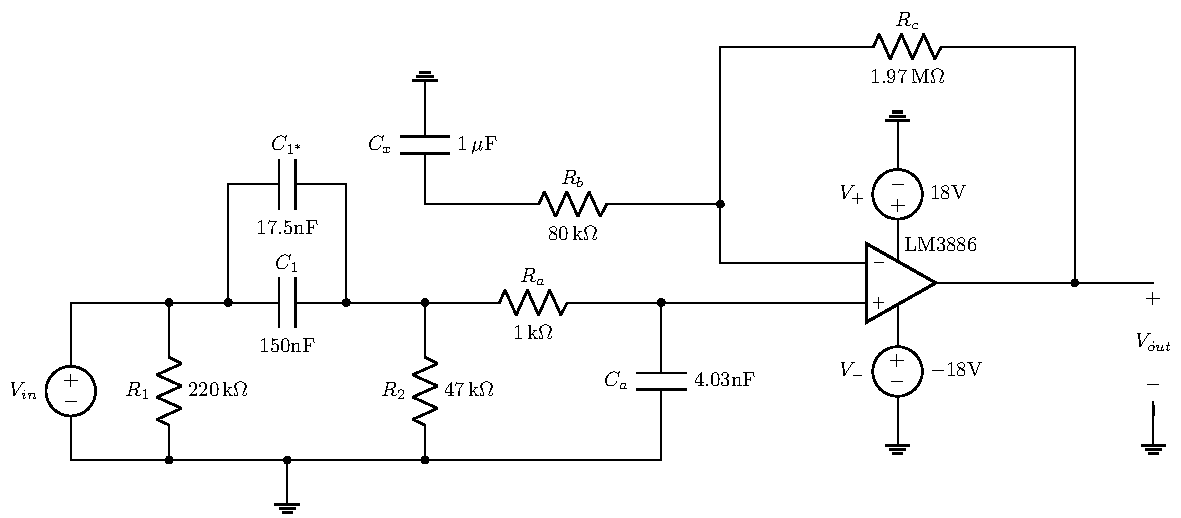
\includegraphics[width=0.9\linewidth]{TU Delft Booming Bass Project Report/figures/PowerAmplifier/circuits/ideal amplifier.pdf}
    \captionsetup{justification=raggedright, labelfont=bf}
    \caption{The ideal power amplifier circuit, where "ideal" refers to the component values leading to a simulation where the frequency response exactly matches the requirements given in \autoref{requirements PA}}
    \label{fig:ideal amplifier}
\end{figure}

To obtain a comprehensive understanding of the circuit's behavior, a frequency sweep from 1Hz to 1MHz was conducted. Simulations of the circuit, using the ideal parameters and values listed in \stautoref{tab:B2-1 ideal values}, indicated that the design requirements were not met (see \sfautoref{fig:not ideal amplifier}). After adjusting the component values to the ideal values in \stautoref{tab: B2-1 actual ideal values}, the bode plot in \sfautoref{fig: ideal amp results} was obtained. The ideal power amplifier simulation utilizes the component values to obtain an ideal frequency response, while the real amplifier operates with the used values from \stautoref{tab: B2-1 actual ideal values}. The frequency response of the real power amplifier is shown in \sfautoref{fig:real circuit results}
\begin{figure}[H]
  \centering
    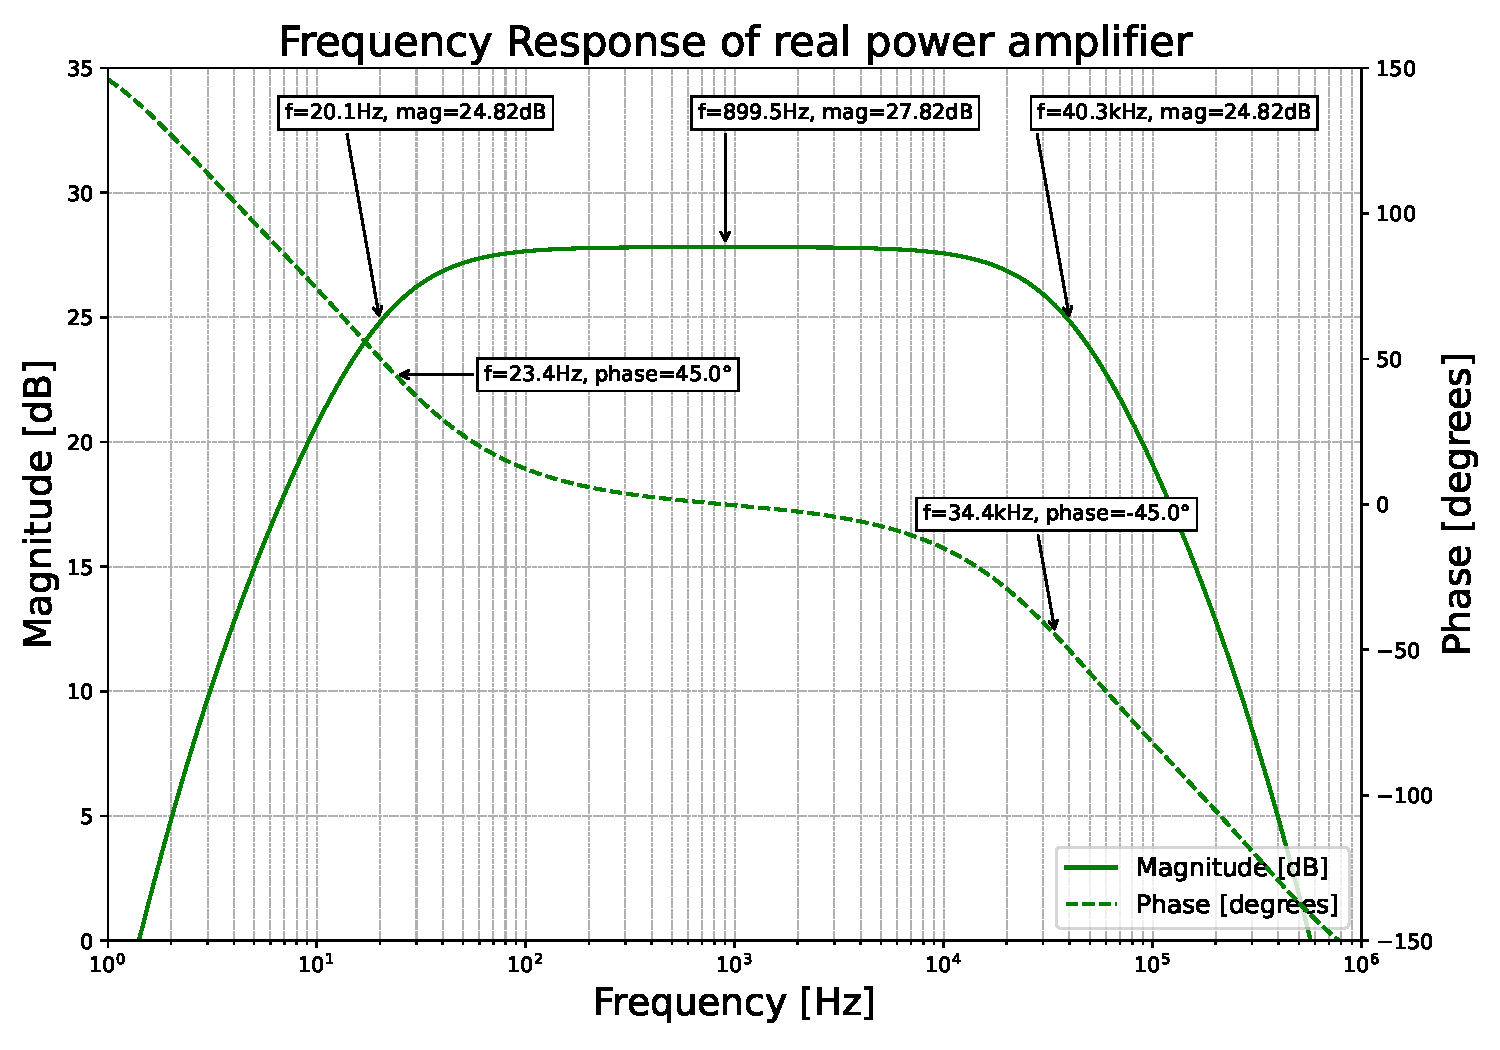
\includegraphics[width=0.75\linewidth]{TU Delft Booming Bass Project Report/figures/PowerAmplifier/real power amplifier results.pdf}
    \captionsetup{justification=raggedright, labelfont=bf}
    \caption{The frequency response of the real power amplifier circuit. As can be seen, the real power amplifier features corner frequencies at around 20.1Hz and 40.3kHz, while maintaining a maximum gain of 27.82dB at a frequency of 899.5Hz.}
    \label{fig:real circuit results}
\end{figure}
\begin{figure}[H]
    \centering
    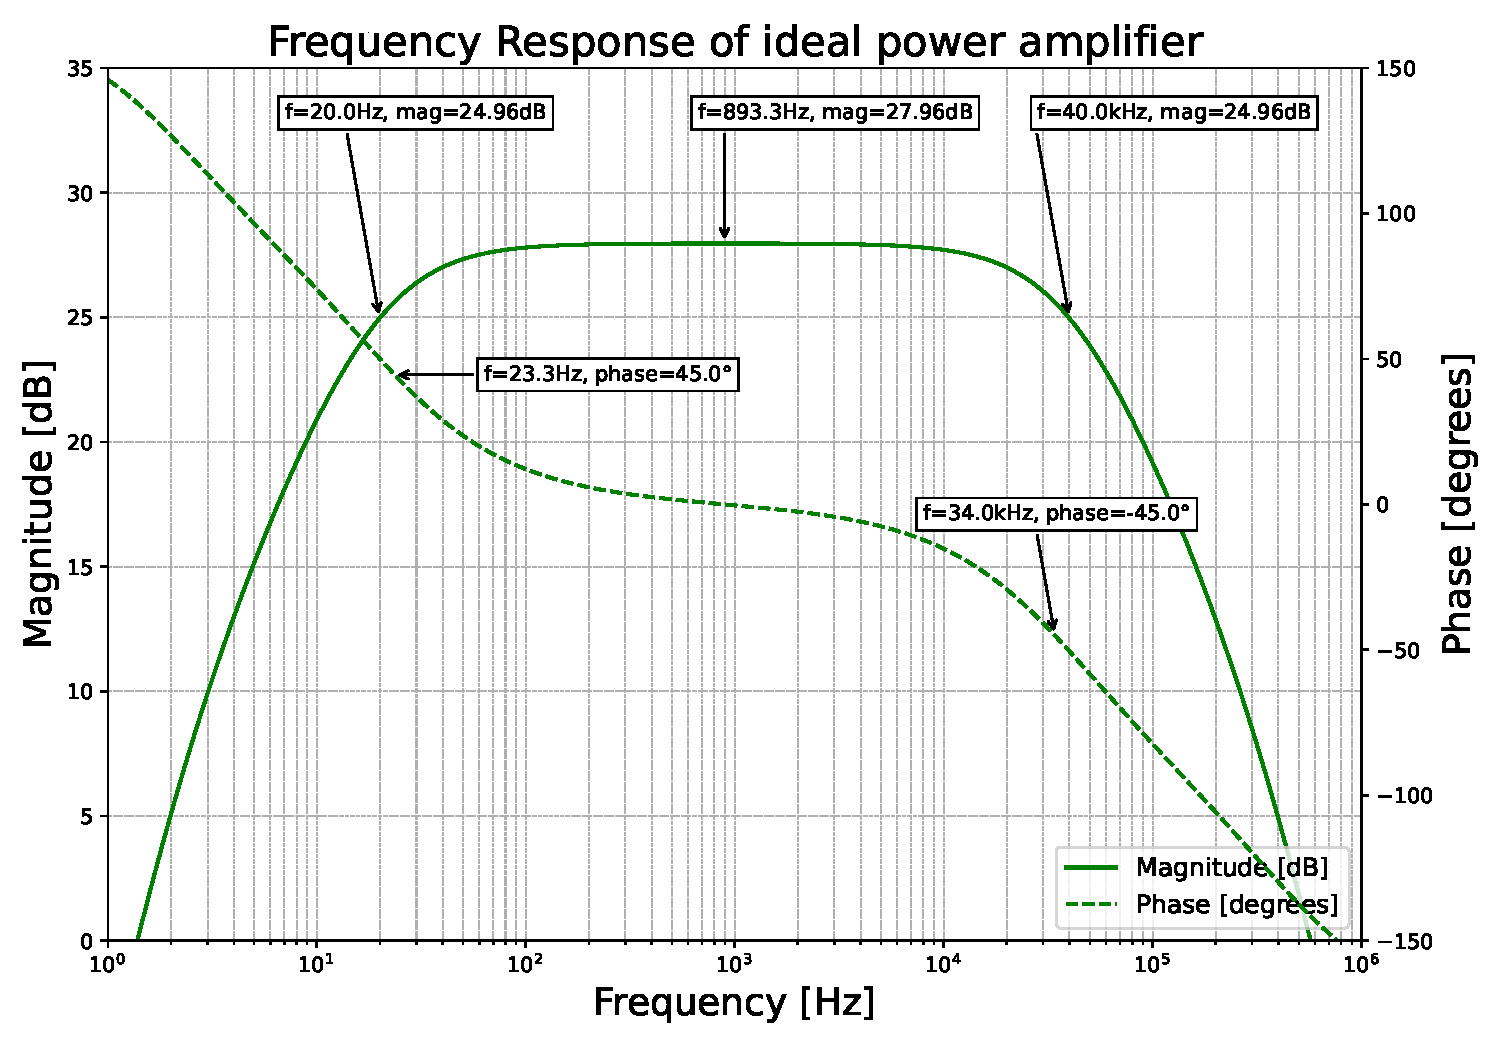
\includegraphics[width=0.75\linewidth]{TU Delft Booming Bass Project Report/figures/PowerAmplifier/ideal power amplifier results.pdf}
    \caption{The ideal frequency response of the power amplifier circuit. As observed, the ideal power amplifier exhibits corner frequencies at 20Hz and 40.0kHz, while maintaining a maximum gain of 27.96dB.}
    \label{fig: ideal amp results}
\end{figure}



\sfautoref{fig: ideal amp results} illustrates that the ideal power amplifier circuit features corner frequencies of 20Hz and 40kHz, with a gain of 27.96dB. In comparison, the real amplifier circuit exhibits corner frequencies of 20.1Hz and 40.3kHz, along with a gain of 27.82dB. In \stautoref{tab: B2-1 actual ideal values}, all of the eventual component values can be seen, along with the deviation between the used values in the real amplifier circuit and both the calculated ideal values and simulated ideal values, respectively.

\begin{table}[H]
    \centering
    \captionsetup{justification=raggedright, labelfont=bf}
    \caption{B2-1 Summary of the calculated ideal values and the corresponding actual-ideal values (Resistance $R_N$, capacitance $C_N$, cut-off frequency $f_{\text{cut-off}}$, and the gain $\mathbf{G_{\text{dB}}}$) based on simulation results. The table includes values for the p-HPF, p-LPF, and a-HPF, with $D_{\text{diff} 1}[\%]$ representing the deviation between the calculated ideal and used values, and $D_{\text{diff} 2}[\%]$ representing the deviation between the simulated ideal and used values.}
    \resizebox{\textwidth}{!}{
    \begin{tabular}{c @{\hspace{12pt}} *7{c} S @{\hspace{12pt}}}
        \toprule
        \multicolumn{7}{c}{\textbf{B2-1 Filter Component Parameters}} \\
        \cmidrule(lr){1-7}
       
        & Parameter & Calculated Value & Ideal Value & Used Value & D$_{\text{diff} 1}$ [\%] & D$_{\text{diff} 2}$ [\%]  \\
        \midrule
        p-HPF & $R_2$ [$\Omega$] & 47k$\Omega$ & 47k$\Omega$ &  47k$\Omega$ &0.00\%  & 0.00\% \\
         & $C_1$ [F] & 169.3nF & 167.5nF &166.5nF & -1.68\%&  -0.60\% \vspace{4pt} \\
         & $f_\text{cut-off}$ [Hz] & 19.8Hz & 20Hz &20.1Hz & 1.50\% &  0.50\% \vspace{10pt} \\
        p-LPF & $R_a$ [$\Omega$] & 1k$\Omega$ &  1k$\Omega$ & 987$\Omega$ & -1.30\%  & -1.30\% \\
         & $C_a$ [F] & 3.98nF & 4.03nF & 4.05nF & 1.76\%& 0.50\%    \vspace{4pt}\\
         & $f_\text{cut-off}$ [Hz] & 40.5kHz & 40kHz & 40.3kHz & -0.50\% & 0.75\% \vspace{10pt}\\
        a-HPF &  $R_b$[$\Omega$] & 80k$\Omega$ & 80k$\Omega$ & 81.8k$\Omega$ & 2.25\% & 2.25\%  \\
        & $R_c$ [$\Omega$] & 1.92M$\Omega$ & 1.97M$\Omega$ & 1.98M$\Omega$ & 3.13\% &  0.51\% \\
         & $C_x$ [F] & 1$\mu$F & 1$\mu$F & 968nF & -3.31\%  &  -3.31\%  \vspace{4pt} \\
         & $\mathbf{G_{\text{dB}}}$  & 27.76dB & 27.96dB & 27.82dB & 0.22\% &  -0.50\%  \\
        \bottomrule
    \end{tabular}
    }
    
    \label{tab: B2-1 actual ideal values}
\end{table}

\subsubsection{Results of B2-2}
As illustrated in \sfautoref{fig: Alternative frequency response output}, using the Used values shown in \autoref{tab:B2-1 ideal values}, the corner frequencies achieved in the simulations for B2-2's design were 20Hz and 36kHz:

\begin{figure}[H]
    \centering
    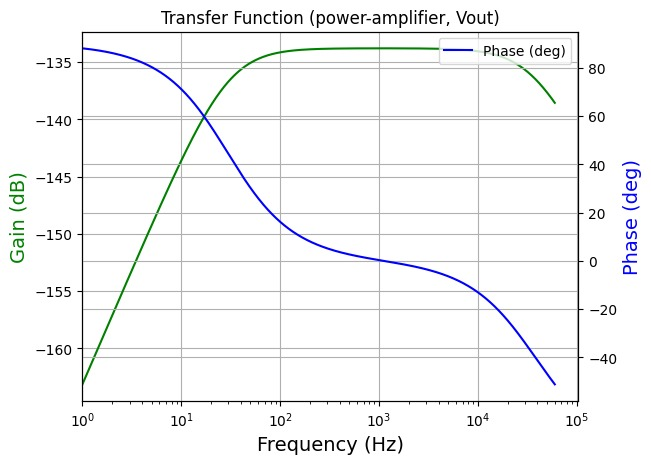
\includegraphics[width=0.75\linewidth]{TU Delft Booming Bass Project Report/figures/PowerAmplifier/Vout alternative design.jpg}
    \captionsetup{justification=raggedright, labelfont=bf}
    \caption{The frequency response of B2-2's power amplifier circuit, with corner frequencies at around 20Hz and 36kHz.}
    \label{fig: Alternative frequency response output}
\end{figure}

\subsection{Filters}
\subsubsection{Simulation of the passive filters}
In order to verify that the calculated component values of the filters produce transfer functions that closely match the desired transfer functions, the designed circuits (\sfautoref{fig:FilterSchematics}) were first individually simulated inside the circuit simulation tool LTSpice. After the individual transfer functions were confirmed to produce the expected results by demonstrating the behavior characteristic of each respective filter. The circuits of all three filters (\sfautoref{fig:FilterSchematics}) with \(R_{ls}\) as the respective speaker's impedance model and with components values from \stautoref{tab:filter_components} were simulated together and tuned further to each other to produce the summed frequency response graph as seen in
\sfautoref{fig:freq_resp}:
\begin{figure}[H]
    \centering
        \begin{minipage}{0.48\textwidth}
            \begin{figure}[H]
            \centering
            \captionsetup{justification=raggedright, labelfont=}
                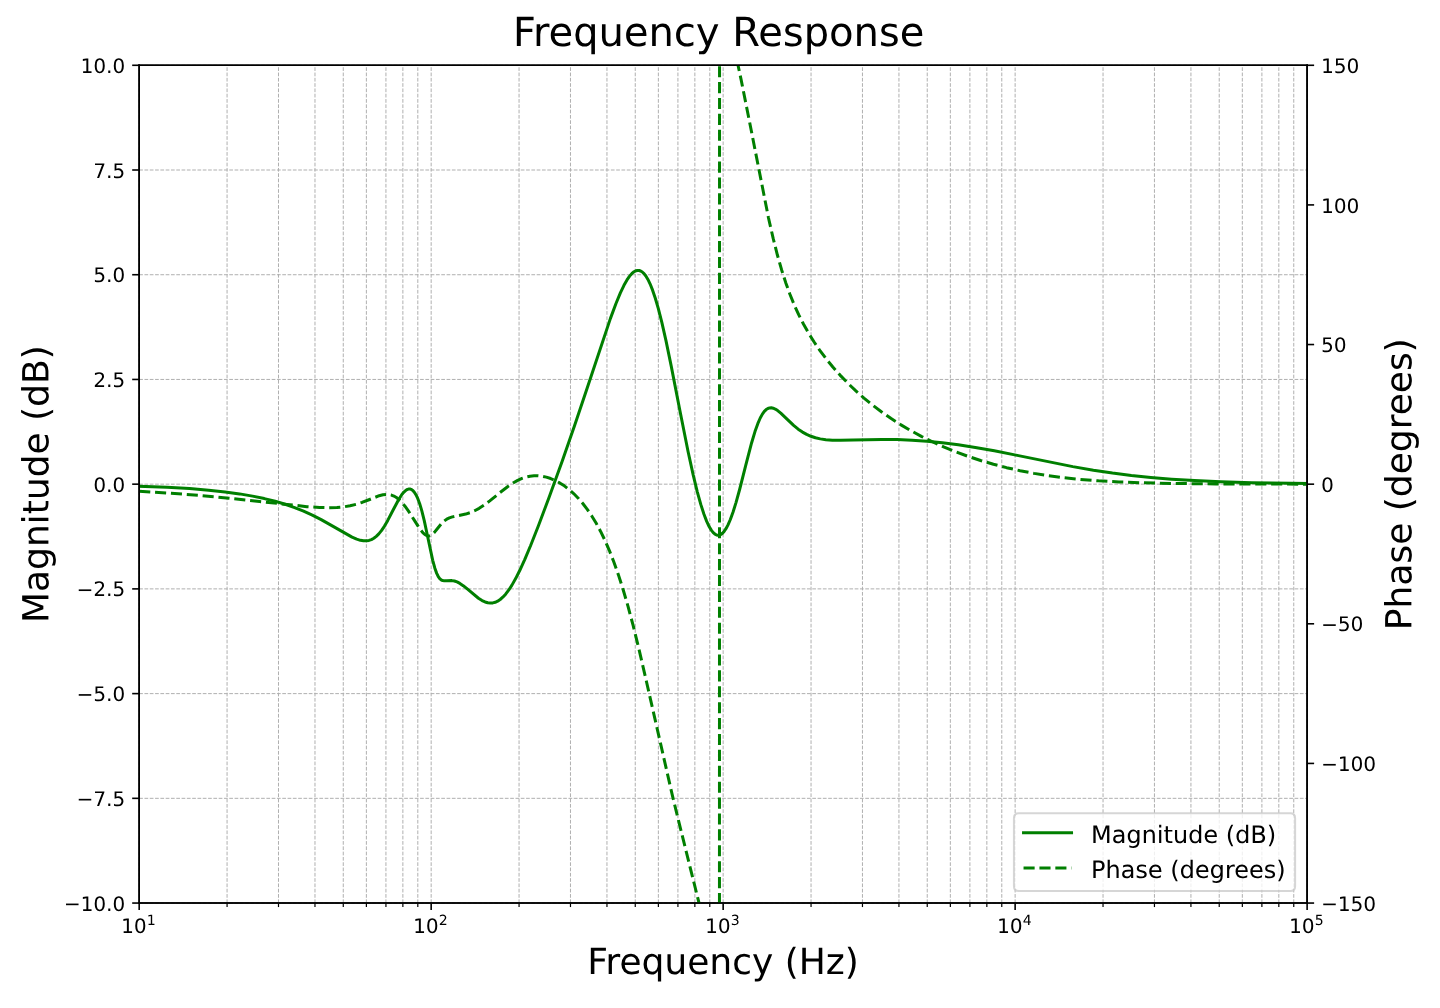
\includegraphics[width=0.9\linewidth]{TU Delft Booming Bass Project Report//figures//FilterGroup/Frequency response.png}
            \caption{Frequency response of the filter bank.}
            \label{fig:freq_resp}
            \end{figure}
        \end{minipage}
        \hfill % Add space between the two mini pages
        \begin{minipage}{0.50\textwidth}
        \captionsetup{justification=raggedright, labelfont=bf}
        \captionof{table}{Values of components for each filter type.}
            \centering
            \begin{tabular}{@{}lccc@{}}
            \toprule
    \textbf{Filter Type}     & \textbf{Component} & \textbf{Value} \\ \midrule
    \multirow{2}{*}{HPF} 
                             & Capacitor                & 28.8 $\mu$F      \\
                             & Inductor                & 0.47 mH        \\ \midrule
    \multirow{2}{*}{Low-Pass of BPF}
                            & Inductor              & 0.67 mH \\
                            & Capacitor             & 100 $\mu$F \\
                            \midrule
    \multirow{2}{*}{High-Pass of BPF}
                            & Capacitor              & 147 $\mu$F \\
                            & Inductor             & 4.7 mH \\
                            \midrule
    
    \multirow{2}{*}{LPF} 
                             & Inductor                & 2.88 mH         \\
                             & Capacitor                 & 100 $\mu$F     \\ \bottomrule
    \end{tabular}
    
        \label{tab:filter_components}
    \end{minipage}
\end{figure}


As seen in \sfautoref{fig:freq_resp}, the frequency response is not     completely flat and has a maximum deviation of 5.0dB at 510Hz; this was found to be acceptable as further altering the values of the components only had a negative effect by shifting the cut-off frequencies to an undesirable range.



\subsection{Loudspeakers}
Using the formulas derived from the circuit model, the corresponding component values can be found for each speaker. The calculations were done for each speaker by their respective filter group, which resulted in the component values found in \stautoref{tab:speaker_components}. 

Using the parameters found, the frequency response of each model was calculated and compared with the measured speaker data. This showed that the model matched closely around the resonance peak but generally had a slightly lower impedance than the measured data, as seen in Fig. \ref{fig:/model vs measured impedance}. 

\begin{figure}[H]
    \centering
    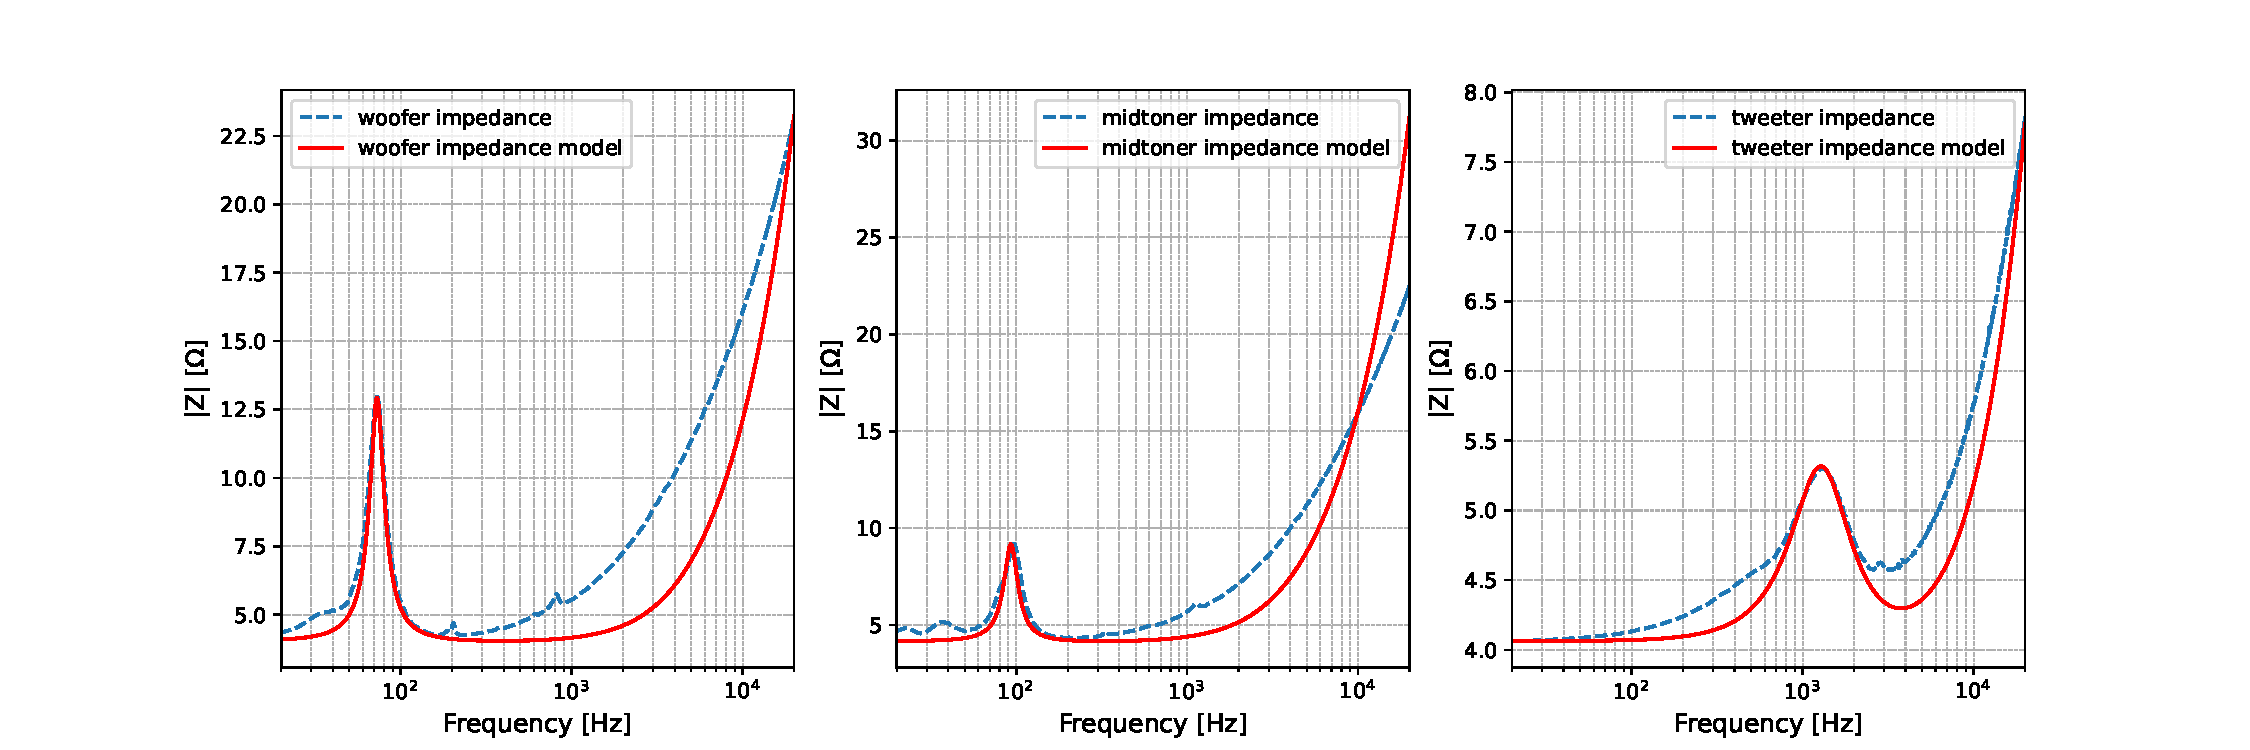
\includegraphics[width=1\textwidth]{TU Delft Booming Bass Project Report/figures/FilterGroup/model vs measured impedance.pdf}
    \captionsetup{justification=raggedright, labelfont=bf}
    \caption{Model speaker impedance versus measured speaker impedance}
    \label{fig:/model vs measured impedance}
\end{figure}

\section{Discussion}

\subsection{Power supply}
The simulations of our circuit are designed to be as accurate as possible. However, since LTSpice may not fully replicate real-world conditions, unexpected differences can arise in practical applications. These discrepancies will be analyzed further in Chapter \ref{subsec:psdiscussion}.


\subsection{Power amplifier}
The circuit with the calculated ideal values probably gives a different result in the simulation than would be expected because LTSpice does take into account the interference between filters, which eventually impacts the frequency response. While in the calculations, all filters were taken separately, as if the interference did not occur. 

The simulations clearly demonstrate that the deviation between the values used in the final circuit is generally closer to the ideal simulated values than to the calculated ideal values. This suggests that the end product is likely to perform in closer alignment with the ideal simulation.

For B2-2's design, it is unclear what the exact amplification is; this may be fixed by using another power amplifier in the simulation. That could be the cause for ending at -135dB. B2-1 used a universal opamp, which did not have this issue.
\subsection{Filters}
During the simulation of the filters, idealized component values were used (e.g. Inductors and Capacitors with no real resistance) as this would greatly simplify the analysis and design process. This clearly differs from real-world circumstances, which would change the transfer function and, thus, the real-life frequency response. 

\subsection{Loudspeakers}
The loudspeaker model is a very simplified version of real-world circumstances. With the entire speaker system being modeled by 5 components, its frequency response will clearly differ from those of the measured speaker data. 

For a more accurate description, a more complex model could have been used, but this, in turn, would have required us to differ from the one in the manual and find or create a new model, and it would have made calculating the model parameters a more arduous task. 